\documentclass[11pt,aps,preprint,nofootinbib,superscriptaddress,tightenlines]{revtex4-2}
\usepackage{amsmath,amssymb,bm,mathtools,graphicx}
\usepackage{xcolor}
\definecolor{darkblue}{RGB}{0,0,160}
\usepackage[colorlinks=true,linkcolor=darkblue,citecolor=darkblue,urlcolor=darkblue]{hyperref}

\def\st{\begin{equation}}
\def\stp{\end{equation}}
\def\Eq#1{eq.~(\ref{#1})}
\def\Sect#1{Sect.~\ref{#1}}
\def\Fig#1{Fig.~\ref{#1}}
\newcommand{\avg}[1]{\langle #1\rangle}
\let\oldparagraph\paragraph
\renewcommand{\paragraph}{\par\bigskip\oldparagraph}

\begin{document}

\title{Frozen or flowing?  How fast SPH particles separate}
\author{D.~Teaney}
\affiliation{Department of Physics and Astronomy, Stony Brook University,
Stony Brook, New York 11794, USA}
\date{\today}

\begin{abstract}
With the smoothed Hamiltonian the SPH particles form a soft solid (transverse sound,
$c_t\simeq0.022$); with the energy representation, at the same temperature, the
transverse correlator is that of a fluid, although at zero temperature the two
Hamiltonians have the same shear modulus.  This note asks what the particles
themselves do: do two neighbours separate in time, and how fast, compared with fluid
elements in fluctuating hydrodynamics?  Campaign \texttt{frozen} measures the separation
of particle pairs together with $C_T$ at three temperatures with \texttt{:energy} and at
one with \texttt{smoothed}.
\end{abstract}

\maketitle

%=============================================================================
\section{The question}
\label{sec:question}

At zero momenta the two Hamiltonians are the same function of the positions,
\st
H\big|_{\bm m=0}=\sum_as_a\,\mathcal E(S_a,0),\qquad S_a=\sum_bs_bW_{ab},
\stp
so the hexagonal lattice has the same static shear modulus in both, $c_t=0.034$ at
$h/a=2$ (\texttt{rigidity.tex}; the deterministic shear wave of \texttt{energystep.tex}
gives the same).  They differ in how the particles move:
\st
\dot{\bm x}_a=\sum_bs_b\Big(\frac{\bm v}{S}\Big)_bW_{ab}\quad(\texttt{smoothed}),\qquad
\dot{\bm x}_a=\bm v_a\quad(\texttt{:energy}).
\label{xdot}
\stp
In the stochastic runs at $\delta v=0.043$ (\texttt{campaigns.tex}) \texttt{smoothed} shows
transverse sound with $c_t\simeq0.022$, \texttt{:energy} none ($c_t\le0.002$).  The question
is whether the arrangement of the particles stays fixed (a solid) or rearranges (a
fluid), and on what time scale.

%=============================================================================
\section{What is measured}
\label{sec:measure}

\paragraph{Displacements.}  Every record (every 2 steps) the driver accumulates the
displacement of each particle from its starting site, without wrapping at the box,
\st
\bm u_a(t)=\bm x_a(t)-\bm x_a(0)-\bar{\bm u}(t),
\stp
with the mean drift $\bar{\bm u}$ removed (\texttt{ParticleRecorder}, \texttt{src/measure.jl}).

\paragraph{Pair separation.}  For the pairs $(i,j)$ that start a distance $r=a$, $2a$, $4a$
or $8a$ apart,
\st
D^2(r,t)=\avg{\,|\bm u_i(t)-\bm u_j(t)|^2\,}_{\rm pairs}.
\label{D2}
\stp
In a solid $D^2$ saturates at a value set by the thermal vibrations.  In a fluid it keeps
growing, in two dimensions as
\st
D^2(r,t)\simeq4D_{\rm rel}(r)\,t ,
\label{D2fluid}
\stp
which defines the relative diffusion constant $D_{\rm rel}(r)$.  The single-particle mean
square displacement $\avg{|\bm u_a|^2}=4D_{\rm self}t$ defines $D_{\rm self}$.  If neighbours
move independently, $D_{\rm rel}=2D_{\rm self}$ for every $r$.

\paragraph{The transverse correlator.}  $C_T(k,\tau)$ as in \texttt{campaigns.tex}, fitted to
the damped oscillator, giving $c_t$ and the damping $2\gamma/\nu k^2$.

%=============================================================================
\section{What a fluctuating fluid would do}
\label{sec:hydro}

A fluid element moves with the local velocity, so two elements separate through the
velocity fluctuations on scales shorter than their distance; longer waves carry both.  In
equilibrium the transverse velocity modes have equal-time variance $T/w$ per unit area
and decay as $e^{-\nu k^2t}$.  The relative velocity of two points a distance $r$ apart
then integrates to
\st
D_{\rm rel}(r)=\frac{T/w}{\nu}\int\frac{d^2k}{(2\pi)^2}\,\frac{1-\cos\bm k\cdot\bm r}{k^2}
\simeq\frac{T/w}{2\pi\nu}\,\ln(k_{\max}r),
\label{Drel}
\stp
and a single element diffuses with
\st
D_{\rm self}\simeq\frac{T/w}{4\pi\nu}\,\ln\frac{k_{\max}L}{2\pi},
\label{Dself}
\stp
with $T/w=\delta v^2V_a$ and the shortest wavelength $k_{\max}\approx\pi/a$.  (The
logarithms are those of two dimensions.  The cutoff is not sharp, since the lattice-scale
modes are not hydrodynamic, so these are estimates to a factor of order one.)  Two
features to test: $D_{\rm rel}$ grows only logarithmically with $r$, and it is set by $T/w$
and $\nu$, so it changes with the temperature.

%=============================================================================
\section{The runs}
\label{sec:runs}

Campaign \texttt{frozen} (\texttt{nersc/campaign\_frozen.txt}; job 61090342, packed on one
node with \texttt{nersc/node.sh}, 32 runs at a time on 4 cores each; code \texttt{main} at
\texttt{1ffc82f}).  All runs: $L=1.2$ ($N=2688$), $h/a=2$, C2, $\eta/s=0.2$, $\lambda=1$, the
equilibrium start, $t=200$, 16 realizations per set.  The entropy density $S_0$ sets the
temperature in units of the particle's own scale, $\delta v=s_a^{-1/2}$; at fixed $\eta/s$ it also
changes $\nu$:
\begin{center}
\begin{tabular}{lcccccc}
\hline
set & $H$ & $S_0$ & $\delta v$ & $\nu$ & $T/w$ & $D_{\rm rel}(a)$, \Eq{Drel} \\ \hline
\texttt{e\_s1e6} & \texttt{:energy} & $10^6$ & $0.043$ & $2.2\times10^{-3}$ & $1.0\times10^{-6}$ & $8.3\times10^{-5}$ \\
\texttt{e\_s1e7} & \texttt{:energy} & $10^7$ & $0.014$ & $1.0\times10^{-3}$ & $1.0\times10^{-7}$ & $1.8\times10^{-5}$ \\
\texttt{e\_s1e8} & \texttt{:energy} & $10^8$ & $0.0043$ & $4.7\times10^{-4}$ & $1.0\times10^{-8}$ & $3.8\times10^{-6}$ \\
\texttt{s\_s1e6} & \texttt{smoothed} & $10^6$ & $0.043$ & $2.2\times10^{-3}$ & $1.0\times10^{-6}$ & $8.3\times10^{-5}$ \\
\hline
\end{tabular}
\end{center}
Analysis: \texttt{examples/frozen\_analysis.jl}.

%=============================================================================
\section{What the runs test}
\label{sec:tests}

\paragraph{A pilot} (debug, box $0.6$, $t=20$, one realization each) already showed the two
extremes at $\delta v=0.043$: with \texttt{smoothed} neighbours barely separate, $D^2(a,20)\approx
0.17a^2$; with \texttt{:energy} they separate about four times faster than \Eq{Drel},
$D^2(a,20)\approx43a^2$, and at the same rate for $r=a$ and $r=8a$, with $D^2\approx2\avg{|\bm
u_a|^2}$: the particles move independently of their neighbours, each with its own thermal
velocity.  The campaign repeats this in the larger box with 16 realizations, and adds the
temperature dependence.

\paragraph{The hypothesis} to test is that with \texttt{:energy} the fluid behaviour comes from
an independent random walk of each particle at the lattice scale, driven by its own thermal
velocity $\delta v$ over a correlation time $\tau_v$,
\st
D_{\rm self}\simeq\delta v^2\,\tau_v ,
\label{walk}
\stp
and that this walk lets the arrangement relax the shear stress, so that the rigidity seen at
zero temperature is lost.  It predicts, as $S_0$ goes from $10^6$ to $10^8$:
\begin{enumerate}
\item $D_{\rm self}$ falls roughly as $\delta v^2$, by about a factor $100$ (if $\tau_v$ does not
  change much), faster than the hydrodynamic estimate, which falls by about $20$.
\item The pair separation stays independent of $r$ while the walk dominates.
\item Once the walk is slow enough that the arrangement does not relax on the time
  scale of the shear mode, $1/\nu k^2$, the transverse sound returns, with $c_t$ approaching the
  static $0.034$.
\end{enumerate}
\paragraph{What would contradict it:} $c_t$ staying at zero at $S_0=10^8$ while the
particles hardly move; or a pair separation at $\delta v=0.043$ that grows like $\ln r$, as in
\Eq{Drel}, rather than being independent of $r$.

\paragraph{The \texttt{smoothed} set} is the reference at $\delta v=0.043$: a solid should show
$D^2(a,t)$ saturating, and $c_t\approx0.022$ as before.

%=============================================================================
\section{Results}
\label{sec:results}

Job 61090342 ran all 64 realizations in 22 minutes on one node.  Diffusion constants are
straight-line fits of $D^2(t)$ and $\avg{|\bm u|^2}$ over $50\le t\le200$, averaged over the 16
realizations (statistical errors about $1$--$3\%$).

\paragraph{1. Do neighbours separate?}  \Fig{fig:D2t}.
\begin{figure}[h]
\centering
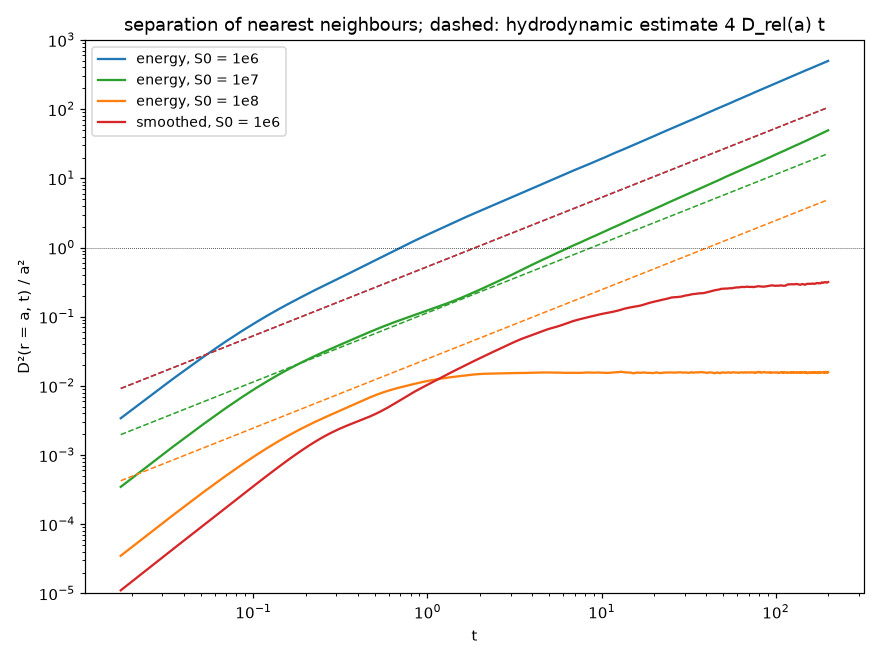
\includegraphics[width=0.75\textwidth]{figs/frozen_D2t.png}
\caption{Pair separation of nearest neighbours, $D^2(a,t)/a^2$ (\Eq{D2}), against $t$, log--log,
mean of 16 realizations.  Dashed, same colour: the fluctuating-hydrodynamics estimate
$4D_{\rm rel}(a)\,t$ of \Eq{Drel} for that set ($\nu$ and $T/w$ differ between the sets; the
two $S_0=10^6$ sets share theirs).  Dotted: $D^2=a^2$.  A line of slope one is a fluid; a
plateau is a solid.}
\label{fig:D2t}
\end{figure}
\begin{itemize}
\item \texttt{:energy}, $S_0=10^6$ and $10^7$: after a short ballistic start ($D^2\propto t^2$)
  $D^2$ grows linearly without bound, reaching $500a^2$ and $50a^2$ at $t=200$.  These are
  fluids: neighbours separate.
\item \texttt{:energy}, $S_0=10^8$: $D^2$ levels off at $0.016a^2$ (a relative vibration of
  $0.13a$) by $t\approx1$ and stays there.  A solid.
\item \texttt{smoothed}, $S_0=10^6$: $D^2$ reaches $0.3a^2$ and is still creeping at $t=200$, but
  about $300$ times below the hydrodynamic line.  A solid, at the same temperature at which
  \texttt{:energy} flows.
\end{itemize}

\paragraph{2. Is the separation that of a fluid?}  \Fig{fig:D2r} and the right panel of
\Fig{fig:summary}.
\begin{figure}[h]
\centering
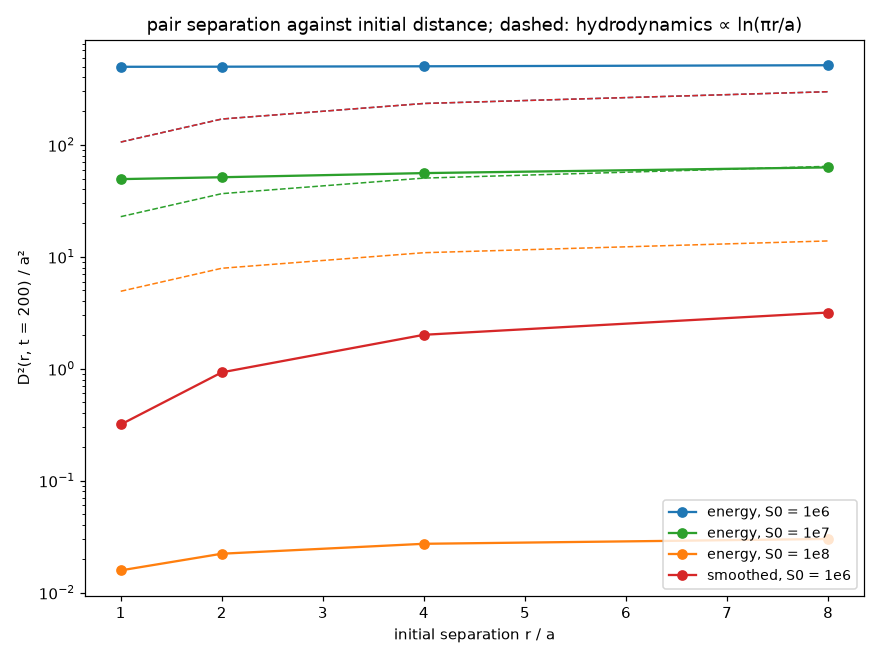
\includegraphics[width=0.7\textwidth]{figs/frozen_D2r.png}
\caption{$D^2(r,t=200)/a^2$ against the initial separation $r/a$.  Dashed: the
hydrodynamic estimate $4D_{\rm rel}(r)\,t$, which grows as $\ln(\pi r/a)$.}
\label{fig:D2r}
\end{figure}
\begin{itemize}
\item $S_0=10^6$ (\texttt{:energy}): $D_{\rm rel}=4.0\times10^{-4}$ for every $r$ from $a$ to $8a$, and
  $D_{\rm rel}=1.95\,D_{\rm self}$.  The particles walk independently of their neighbours, $2$--$5$
  times faster than fluid elements would ($D_{\rm rel}(a)$ is $4.9$ times \Eq{Drel},
  $D_{\rm self}$ is $1.8$ times \Eq{Dself}).  This is the random walk of \Eq{walk}, with
  $\tau_v=D_{\rm self}/\delta v^2=0.11$.
\item $S_0=10^7$ (\texttt{:energy}): $D_{\rm rel}$ rises with $r$, from $4.1$ to $5.0\times10^{-5}$,
  and approaches the hydrodynamic value: the ratio to \Eq{Drel} is $2.3$, $1.5$, $1.1$, $1.0$ at
  $r=a$, $2a$, $4a$, $8a$, and $D_{\rm self}$ is $1.1$ times \Eq{Dself}.  Close to fluid
  elements, with an excess of independent motion only at the shortest distance.
\item The two \texttt{:energy} fluids differ by a factor $10$ in $D_{\rm rel}(a)$, the ratio of
  $\delta v^2$ (hydrodynamics would give $4.6$).  The walk scales as $\delta v^2$ there
  ($\tau_v=0.11$ and $0.15$).
\end{itemize}

\paragraph{3. Does the transverse sound come back when the particles freeze?}  \Fig{fig:CT}
and the left panels of \Fig{fig:summary}.
\begin{figure}[h]
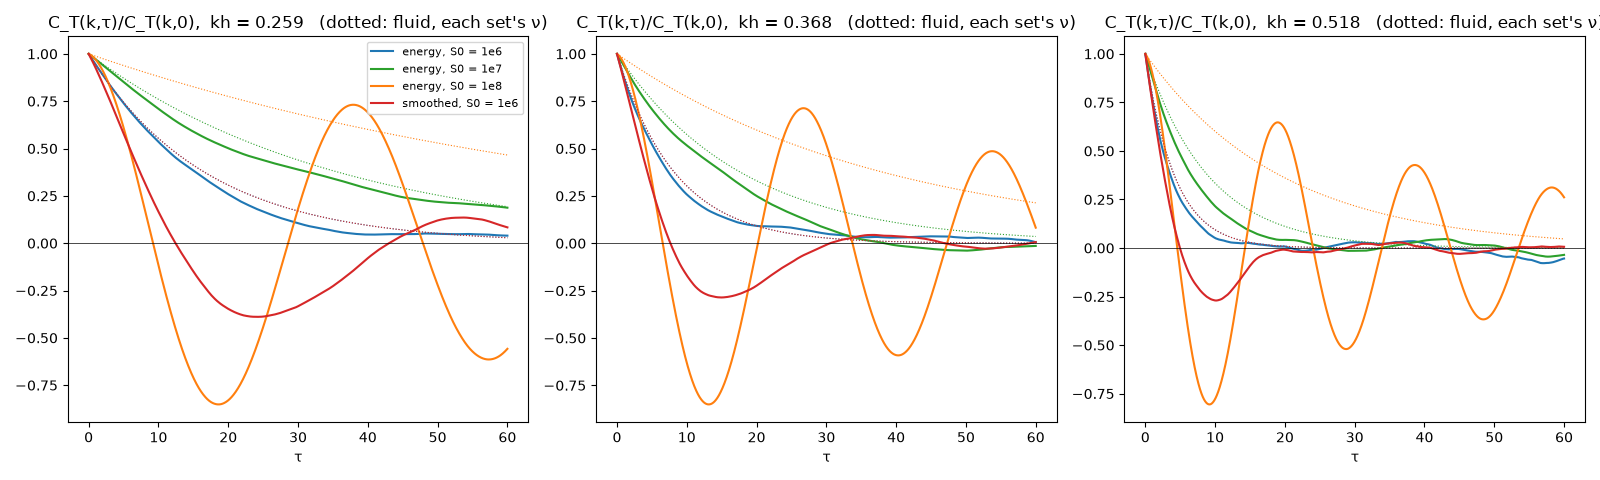
\includegraphics[width=\textwidth]{figs/frozen_CT.png}
\caption{$C_T(k,\tau)/C_T(k,0)$ in three shells, the four sets; dotted, the fluid
$e^{-\nu k^2\tau}$ with each set's $\nu$.}
\label{fig:CT}
\end{figure}
\begin{figure}[h]
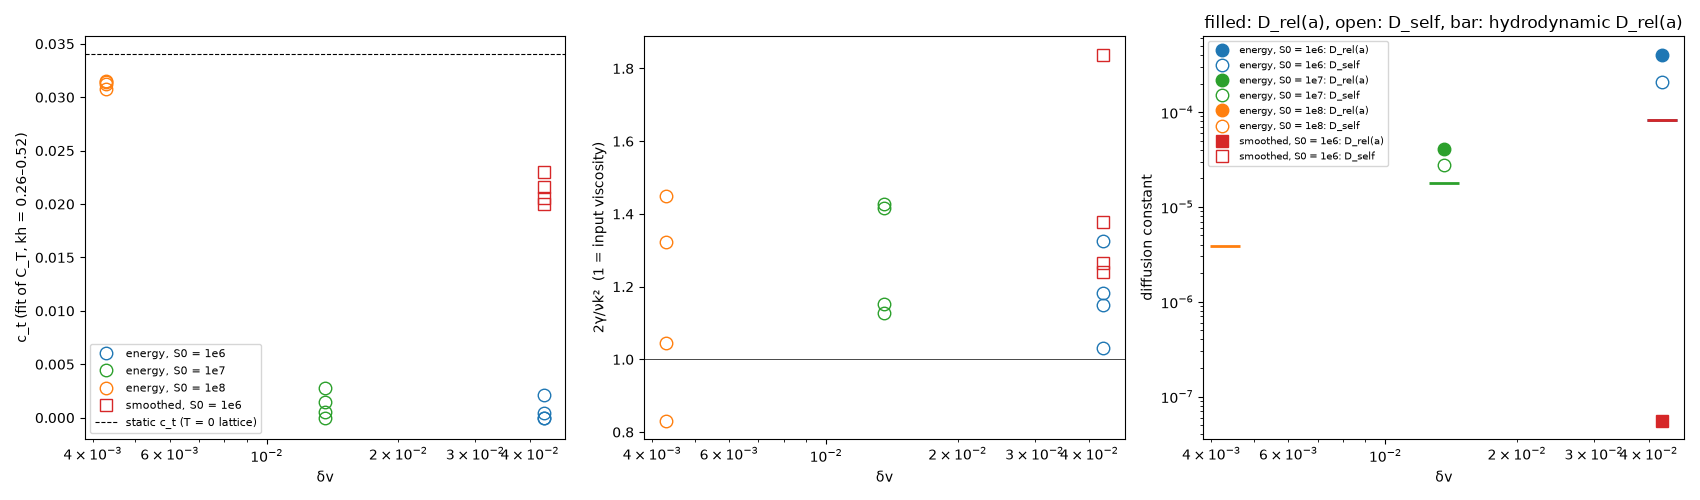
\includegraphics[width=\textwidth]{figs/frozen_summary.png}
\caption{Against $\delta v$, one point per shell ($kh=0.26$--$0.52$).  Left: $c_t$ from the fit
of $C_T$, with the static value $0.034$ of the $T=0$ lattice (dashed).  Middle: the damping
$2\gamma/\nu k^2$.  Right: $D_{\rm rel}(a)$ (filled) and $D_{\rm self}$ (open) with the
hydrodynamic $D_{\rm rel}(a)$ (bar); the frozen sets are off scale below ($|D|<10^{-9}$ for
\texttt{:energy} at $10^8$).}
\label{fig:summary}
\end{figure}
Yes.  \texttt{:energy} at $S_0=10^8$ oscillates strongly in every shell with
$c_t=0.031$, close to the static $0.034$; at $10^6$ and $10^7$, where the particles flow,
$c_t=0.000$--$0.003$.  \texttt{smoothed} at $10^6$ gives $c_t=0.020$--$0.023$, as in all earlier
runs.  The damping is $1.0$--$1.45$ times the input in all sets.  The transverse sound
goes with the frozen arrangement, and is absent exactly when neighbours separate.

\paragraph{4. Energy.}  \Fig{fig:energy}.
\begin{figure}[h]
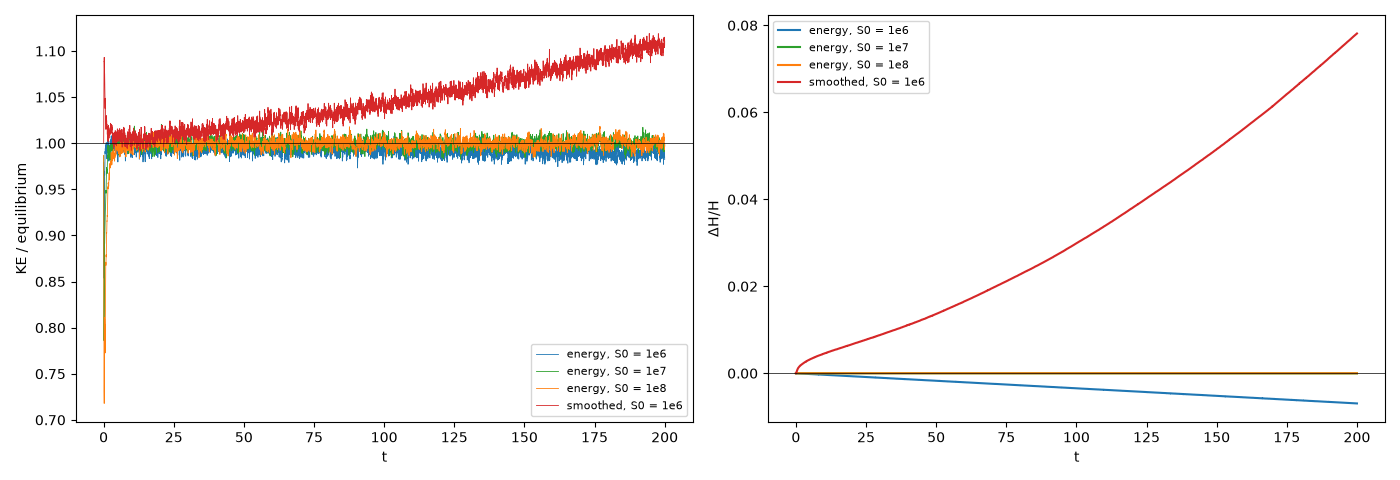
\includegraphics[width=\textwidth]{figs/frozen_energy.png}
\caption{KE/eq and $\Delta H/H$ against $t$, mean of 16 realizations.}
\label{fig:energy}
\end{figure}
KE/eq is $0.99$--$1.00$ for every \texttt{:energy} set; \texttt{smoothed} heats as before
($\Delta H/H=+7.8\times10^{-2}$, KE/eq rising to $1.10$).  The linear loss of \texttt{:energy}
falls steeply with temperature, $\Delta H/H(200)=-6.9\times10^{-3}$, $-3.2\times10^{-5}$,
$-1.4\times10^{-7}$ at $S_0=10^6$, $10^7$, $10^8$: a factor $\approx220$ per decade of $S_0$,
roughly $\delta v^{4.7}$.  It is there in the frozen set too, so it is not caused by the
particles flowing.

%=============================================================================
\section{Conclusions}
\label{sec:conclusions}

\begin{enumerate}
\item \emph{The transverse sound is the rigidity of a frozen particle arrangement, and it
  disappears when the arrangement melts.}  With \texttt{:energy} the particles form a solid at
  $\delta v=0.0043$ ($c_t=0.031$, neighbours vibrate by $0.13a$ and never separate) and a fluid at
  $\delta v=0.014$ and $0.043$ ($c_t\approx0$, neighbours separate diffusively).  The melting lies
  between $\delta v=0.0043$ and $0.014$ at $h/a=2$.
\item \emph{With \texttt{smoothed} the arrangement stays frozen at $\delta v=0.043$,} where
  \texttt{:energy} flows, and three times hotter in $\delta v$ (ten times in $T/w$) than the
  coolest set at which \texttt{:energy} is already fluid.
  Its particles move with the smoothed velocity, \Eq{xdot}, which leaves neighbours almost no
  relative motion; this is why the two Hamiltonians, with the same static modulus, behave so
  differently.
\item \emph{How fast particles separate.}  At $\delta v=0.014$ the \texttt{:energy} particles
  separate like fluid elements of fluctuating hydrodynamics, within a factor $2$ at $r=a$ and
  within $10\%$ at $r\ge4a$, with no fitted parameter.  At $\delta v=0.043$ they walk
  independently of their neighbours, $2$--$5$ times faster than fluid elements: there the
  particle-level noise, not the hydrodynamic flow, moves them.
\item \emph{So, for \texttt{:energy} at $h/a=2$, there is a window in $\delta v$} in which the
  particles are a fluid that moves like one.  Below it they freeze into a solid; above it
  their individual thermal motion dominates.  The window's location will depend on $h/a$,
  since the static rigidity falls with $h/a$ (\texttt{rigidity.tex}).
\item The loss of energy with \texttt{:energy} is unrelated to the flow and falls roughly as
  $\delta v^{4.7}$; at $\delta v=0.014$ it is $-3\times10^{-5}$ over $t=200$.
\end{enumerate}

\paragraph{Open, and possible next runs.}
\begin{enumerate}
\item Locate the melting: $S_0=2\times10^7$, $3\times10^7$, $5\times10^7$ with \texttt{:energy}.
  Check for hysteresis by starting at $10^8$ from a melted arrangement.
\item The window against $h/a$ ($2.5$, $3$) and the kernel.
\item Does \texttt{smoothed} ever flow at higher $\delta v$ (where it heats and becomes unstable,
  \texttt{campaigns.tex})?
\item The $L=2.4$ box at $\delta v=0.014$ with \texttt{:energy}, where the fluid looks closest to
  hydrodynamics: $C_T$ against $e^{-\nu k^2\tau}$ down to $kh=0.13$.
\end{enumerate}

\end{document}
